\title{{\bf Alberta's Oil Sands EROI Multi-Objective Optimization (MOP)}}
\author{
          MIT Precision Engineering Research Group (PERG)\\
	  }
\date{August 9th, 2015}

\documentclass[12pt]{article}
\usepackage{fancyhdr}
\usepackage{amsmath}
\usepackage{amssymb}
\usepackage{amsthm}
\usepackage{color}
\usepackage{graphicx}
\usepackage{enumerate}
\usepackage{lastpage}
\setlength{\textwidth}{5.5in}
\setlength{\textheight}{8.5in}
\setlength{\voffset}{-0.5in}
\setlength{\hoffset}{-0.2in}
\newcommand{\h}[1]{\colorbox{yellow}{#1}}
\renewcommand\headrule{}
\definecolor{ashgrey}{rgb}{0.7, 0.75, 0.71}
\pagestyle{fancy}

\begin{document}
\lhead{}
\chead{\color{ashgrey}{DRAFT 2015-08-09}}
\rhead{}
\lfoot{}
\cfoot{Page \thepage\ of \pageref{LastPage}}
\maketitle

\begin{abstract}
The province of Alberta is operating on a poor Energy Return on Investment (EROI). In this paper, we believe we can improve EROI by evaluating different renewable system models  from a Single-Objective Optimization (SOO) and Multi-Objective Optimization (MOP) approaches.  
\end{abstract}

\tableofcontents
\newpage

%%%%%%%%%%%%%%%%%%%%%%%%%%%%%%%%%%%%%%%%%%%%%%%%%
\section{Introduction}
%%%%%%%%%%%%%%%%%%%%%%%%%%%%%%%%%%%%%%%%%%%%%%%%%

\subsection{Problem Domain}

{\bf Context} \\

The development of the oil sands industry has experienced two challenging events in the past months. First, the continous drop of oil price and, second,  the rejection of Keystone XL by the Obama administration. As a consequence, oil companies have started to pull the plug on Alberta expansions and cutting down the expenses under a break-even threshold analyst say is needed to justify a bran new oil sand expansion. Furthermore, companies are trimming spending plans and reducing workforces in response.  Poisson et al [ref] states that Alberta is operating at a poor return per investment. Within this context, two important questions arise: 
  \begin{enumerate}
  \item How could producers be more efficient and develop new technologies that lower production and maintenance costs?
  \item How could companies cut costs and eliminate inefficiencies in the industry
  \end{enumerate}

In this paper, we hope to provide some insights to these questions by evaluating Alberta's Energy Return on Investment (EROI) from a single-objective optimization and multi-objective optimization approaches. \\

\subsection{Introduction to Optimization}

\begin{itemize}
\item classical optimization concept for a single-variable
\item classical optimization concept for multi-variables
\item single and multi objective optimization
\end{itemize}

\subsection{Algorithms}

We provide a general overview of the algorithms we implement in this paper as a basic reference of their running time and implementation.

Optimization Algorithms
\begin{itemize}
\item Branch and Bound
\item Tabu Search
\end{itemize}

Approximation Algorithms
\begin{itemize}
\item
\end{itemize}

\subsection{Current Supply \& Demand}

Current studies show that there is presently more supply than demand for the oil industry. In this paper, we are interested in studying supply versus deman from supply need point of view defined as the actual supply need from the oil sands to generate energy. The price of oil has been fluctuating a lot in the past months, yet people basic needs have been evolving more slowly. The price of gas is not considerably lower and we want to address the issue of  supply from a concrete need of the population. We will talk about elastic and inelastic demand. \\

The price for a barrel was above US\$100 in 2013 [2], however, companies were making their highest profits back in 2007 when the price of a barrel of oil was US\$54 [3]. Therefore, industries were making four times as much profit was they were making it today. As the price of a barrel of oil went up, so did all the supplier costs and third party services. Now, the price has significantly dropped, but the cost of suppliers and other vendors have remained the same. \\

\begin{center}
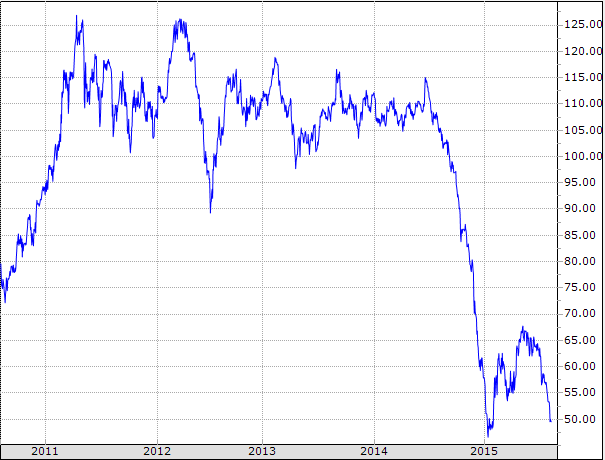
\includegraphics[scale=0.65]{oilprices.png}
% Graph coming from MoneyAM.com
% Retrieved on August 7, 2015
\end{center}

\subsection{Motivation}
In this paper we study Alberta's oil sands EROI as a multi-objective optimization problem in order to show that if we were to use renewables as a symbiotic approach for the development of oil sands as describe in [1], then not only we can achieve a carbon-neutral industry, but also a more profitable industry that can benefit both the government and oil producers. \\

In this paper, we will focus on: 

\begin{enumerate}
\item {\bf Modelling} 

\begin{itemize}
\item We create a basic model.  
\item We feed the model input parameters
\item We generate a complete model which we will then test. We will not know if the model created is useful or not, so we perform optimization analysis to figure out. 
\item Explain the WHY of the model. What question does it answer?
\end{itemize}

How is this useful/effective? According to what criteria? How to justify this criteria? 

\item {\bf Simulating} 

\begin{itemize}
\item We identify different scenarios described by the model we built 
\item We simulate those senarios to test if the new configuration is better thant the conventional configuration
\item Simulate on different objectives and see. Conclude different propositions as a result.
\end{itemize}

\item {\bf Optimazing} 
\begin{itemize}
\item Based on the configuration, we identify the most important factors, variables, and which elements take into account. 
\item We test the configuration with all optimization algorithms to find a set of pareto optimal solutions
\item If no solution is found, explain why
\end{itemize}
\end{enumerate}

The research within the oil sands industry is a complex Minimizing/Maximizing optimization problem where we are trying to minimize the CO$_2$ amount while maximizing profits. It combines solutions from Discrete, Combinatorial, Stochastic, and Multi-Objetive algorithms. \\

In this paper, we discuss the combination of multiple methods to find a better configuration than the conventional configuration through meta-huristic algorithms. \\

\begin{center}
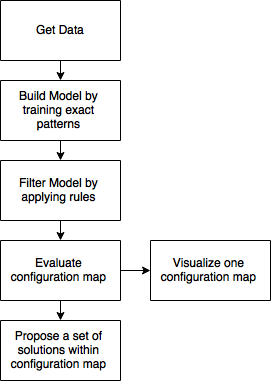
\includegraphics[scale=0.75]{dataflow.png}
\end{center}

\subsection{Methods}

Methodology:
\begin{enumerate}
\item First Approach: Brute-Force. Find out how much time it takes for the computer to find a solution. If we need to change a specific variable (say the price of oil again), then it will take again a certain amount of time to solve. 
\item Second Approach: try to cut down the time by a more global approach: 1) Branch and Bound 2) Tabu Search . We will test how this evolves and how different scenarios produce different solutions through these methods. 
\item Third Approach: test in parallel all Meta-Heuristics: 1) VEGA 2) TAPAS 3) ETC. 
\item Final Approach: take approximate solutions to approximate problems. (Provide more details)

\end{enumerate}


%%%%%%%%%%%%%%%%%%%%%%%%%%%%%%%%%%%%%%%%%%%%%%%%%
\section{Modelling}
%%%%%%%%%%%%%%%%%%%%%%%%%%%%%%%%%%%%%%%%%%%%%%%%%

\subsection{Model Generation}

We address the Oil Sands EROI problem from the following perpective: \\

{\bf Definition:} Define $B$ the cost of a barrel of oil in the market, $E$ the energy required to develop a barrel of oil (need to clarify what this means), $C$ the cost of producing 1 barrel of oil with a given method, $P$ the profit made by the oil company exploiting the bitumen,  $M$ the maintenance, and $X$ the amount of CO$_2$ released to the atmosphere to produce such barrel. of oil We want to model the following cost vector $v$ as a multi-objective optimization problem:

\begin{displaymath}
v = \langle B, E, C_B, P,  M, X \rangle
\end{displaymath}

We specify what we mean by $P$. If different companies have different profits then we talk about another vector of prices, different companies have different prices associated with the geo location region they work on, hence $P$ is also a cost vector defined as 
\begin{displaymath}
P = \langle R, \#bbl, T \rangle
\end{displaymath}
Where $R$ is the associated region the oil company works, $\#bbl$ is the number of barrel of oil produced within $T$ days

We want to study this cost vector $v$ based on different scenarios (or weights on different variables)and different methods of producing a barrel of oil using renewables. Depending on our decisions, we will weight some variables more than others. This vector $v$ will serve more and an indicator of performance for different EROI models. As an analogy, consider how different organizations provide university rankings based on different criteria (number of PhDs, research grants, Nobel Prize winners, etc), this vector will behave in a similar basis.  Changing variable weights will return different solutions for different scenarios. \\

This EROI analysis We can bring this discussion to the table. If we agree to weight into a certain variable more than another one, we the domocratically judge what model to focus on based on which multi-objective function. This will clarify the choices of the model we will expand our work on. It will come down to how we weight these variables in question that will define the best working model for the problem. Ultimately, there is no mathematics that does this, it will depend on human decisions. \\

In this paper, we analyze the EROI problem through different situations to find which variables do we have control over, which variables we do not have control over (paramaters and coefficients), and which variables we want to optimize. In this paper, we want to show that the vector 

\begin{displaymath}
v_{wind+solar}= \langle B, E_{wind} + E_{solar}, C_{wind} + C_{solar}, P_{wind + solar}, X_{wind+solar}\rangle
\end{displaymath}
 yields better EROI while proving to be a good solutions towards a carbon-neutral future for Alberta. \\

In other words, we want the following linear combination:

\begin{displaymath}
P_{wind+solar} = \underbrace{\alpha \times E_w \times C_w}_\text{EROI Wind Energy} + \underbrace{ \beta \times E_s \times C_s}_\text{EROI Solar Energy}
\end{displaymath}

In this paper we show that $\beta \times E_s \times C_s \approx 0$ does not yield a good EROI, hence $P \approx \alpha \times E_w \times C_w $\\

\subsection{Input Parameters}

To study a more detailed model, we allo input parameters in our backbone model such as:
\begin{itemize}
\item Peak Power of wind turbine
\item Peak Power of solar panel
\item Reinvestment policy into buying more wind turbines or more solar powers
\item Cost per Watt
\end{itemize}

\subsection{Complete Model}

We provide a more detailed cost vector function. 

%%%%%%%%%%%%%%%%%%%%%%%%%%%%%%%%%%%%%%%%%%%%%%%%%
\section{Simulation}
%%%%%%%%%%%%%%%%%%%%%%%%%%%%%%%%%%%%%%%%%%%%%%%%%

\subsection{Algorithm Design}

We want to:
\begin{itemize}
\item Design and Development of an Algorithm
\item Run and test this algorithm
\end{itemize}

\subsection{Techniques}

\begin{itemize}
\item The first approach will be by exahustive enumeration (brute force). 
\item Second approach is a branch and bound approach where we are interested in cutting down the number of cases to consider in a decision tree. To explore the heuristics, we take this variable in the grid. We try with another variable. Some discrete variables can be used as continuous. 
\item We try to find a pareto optimal. But first, we go by scenario-approach. We look for pareto local solutions. We look at different pareto local solutions based on different scenarios. Looking at the model, we might introduce new constrains that we never though before. This process allows to illicit their contrains or needs depending on the choices we make. Then, we can possible arrive at a pareto optimal solution. 
\end{itemize}

\begin{enumerate}
\item Using generic algorithms (meta-heuristics)
\item Non-scalar and non-pareto approch: VEGA (Vector Evaluated Genetic Algorithm)
\item Target Amining Pareto Search (TAPAS)
\item Path Relinking Algorithm: Neighborhood Exploration. Add graph.
\item  Path Linking Method. We look at the neighborhood of the solution space. 2-objective functions gives birth to 2 grids. Cube space (a,b,c) a = Wind, b = Solar, c = Mining. Different configurations can represent something interesting things. Our topology map will be encoded based on our contrains. Then we need to establish rules, for instance, (1,1,0) can be next to (1,0,1), but not next to (0,1,1) we encode the solution structure. Given X, this is the neighborhood.  
\item Domination Dependent lifetime: maximal lifetime is assigned to each wind turbine. The lifetime is shortened if the solution dominates a major part of the present non-dominated solutions. This limits the impact of the solution. 
\end{enumerate}

%%%%%%%%%%%%%%%%%%%%%%%%%%%%%%%%%%%%%%%%%%%%%%%%%%
\section{Optimization Analysis}
%%%%%%%%%%%%%%%%%%%%%%555555%%%%%%%%%%%%%%%%%%%%%%%%

A multi-objective optimization problem consists in a set of objectives (discrete variables) to which we associate a cost function we want to optimize. The set of optimized solutions is the pareto optimal set. \\

In the pursuit of finding a pareto optinal solution, we will study different pareto optimums which represent different choices because our cost vector  $v$ does not have more information. We give the pareto optimum solutions scenarios, we cannot distinguish them if we don't weight in some variables more than others, so we are left with a choice. Then, based on that choice, we will show what we have found. \\

\subsection{Discrete Optimization}
The configuration network is a discrete because the choice of putting a turbine or not is also
discrete (yes or not). \\

how many do we place? a bit less a bit more? amortize it.

\subsection{Cominatorial Optimization}
There're many heuristics exist for this type of problem such as Tabu Search or the Genetic Algorithm, in concrete it is a problem with complex structural optimization.  

\subsection{Stochastic Optimization}
When talking about the functioning of the turbine, there are data problems. Here we can talk about machine learning because the turbine needs to learn when to shut down when there is no wind. This is stochastic optimization problem. We have a real system where the wind is random variable, we have the choice of keeping the turbine on or to turn it off, and if we don't do this at the right time, turbine could be non-functioning anymore. \\ 

\subsection{Multi-objective optimization}
we want to maximize something and minimize something. Is there a direct relationship?
Maybe be not. This what we call multi-objective optimization (profit, CO$_2$). When we have conflicting variables, there are artificial trade-offs.  \\

CO$_2$ evaluation methods are highly political. Need to play with this 2 tables (profit, CO$_2$)

\subsection{Performance Assessment}
\begin{itemize}
\item How to measure the quality of the solution? 
\item How much time does it take to generate the solution set?
\item What we find in this paper is that we don't find a single solution, but rather a set of solutions based on trade-offs
\end{itemize}


%%%%%%%%%%%%%%%%%%%%%%%%%%%%%%%%%%%%%%%%%%%%%%%%%
\section{Results}
%%%%%%%%%%%%%%%%%%%%%%%%%%%%%%%%%%%%
\subsection{EROI Models}

{\bf CO$_2$ Neutral solution long term}
\begin{itemize}
\item More progress towards land reclamation. 
\end{itemize}


{\bf Sample results;;}
\begin{itemize}
\item More \$ for refineries and pipelines
\item (SAMPLE) The technology resulted in an additional 1,600 barrels of bitumen per day being recovered from just one vessel. The figure means that 50\% less marerial ends up in tailing ponds, and at oil prices \$50 per barrel translates into an additional 30 million in annual revenues for Suncor. 
\end{itemize}

%%%%%%%%%%%%%%%%%%%%%%%%%%%%%%%%%%%%%%%%%%%%%%%%%
\section{Conclusion}
%%%%%%%%%%%%%%%%%%%%%%%%%%%%%%%%%%%%%%%%%%%%%%%%%
The big picture: what do we propose? and to whom do we propose to? Then a several things to consider. \\

We proposed the EROI problem from a multi-objective optimization problem. We showed what can we generate different models based on input parameters. We showed that those created models represent different scenarios (or configurations) which could give a set of solutions or not. 

If there is something in these results that is of interest to the energy sector we then plan to expand on that specific branch and show what has to be done for that to happen.\\  

We showed that this set of configurations performs better than the conventional configuration in terms of EROI provided the simulation scenarios. \\

The difference with this problem and other problem in industry is that at the end of the day we have a choice. We can go further and propose things to politicians and oil companies. We can propose things, see how the problem is approached,  and find a better balance between profit margins and public safety . \\

Process:
End user action focusing $\rightarrow$ High Order Complex relationship $\rightarrow$
Transparency (Provide an easy way to understand outcomes  instead of black box approaches) $\rightarrow$ Multiple Data Sources (handling Unstructured data) 

\newpage

%%%%%%%%%%%%%%%%%%%%%%%%%%%%%%%%%%%%%%%%%%%%%%%%%
\section{References}
%%%%%%%%%%%%%%%%%%%%%%%%%%%%%%%%%%%%%%%%%%%%%%%%%

[1] Slocum et al. \emph{A Symbiotic Approach for the Development of Oil Sands.} \\

\noindent [2] Smith, Aaron. \emph{Oil prices at 2013 high above \$103 a barrel}. Retrieved on June 29, 2015 from http://money.cnn.com/ \\

\noindent [3] Tencer, Daniel. \emph{CNRL's Steve Laut Says Oilsands Face 'Death Spiral' If They Don't Cut Costs}. Retrieved on February 19, 2015 from http://www.huffingtonpost.ca/


\end{document}
